\section{Linear Time-invariant DAEs}

\subsection{System Theoretic Aspects of DAEs}
Consider
\begin{align*}
	Ex(t) &= Ax(t) + Bu(t), \quad x(0) = x_0, \\
	y(t) &= Cx(t),
\end{align*}
where
\begin{itemize}
	\item $x(t) \in \Rn$: the system's state
	\item $u(t) \in \Rm$: the input or control
	\item $y(t) \in \Rq$: the output or measurements
	\item $E \in \Rnn$ is \emph{singular}
	\item $A \in \Rnn$: the system matrix
	\item $B \in \Rnm$: the input matrix
	\item $C \in \Rqn$: the output matrix
\end{itemize}
we will denote the system by \eabcsys.

Often, these \eabcsys~are referred to as \emph{descriptor} or \emph{singular} systems.

The transfer function of an \eabcsys~in time domain is given as
	\begin{align*}
		&\mathbf G \colon u \mapsto y\colon\\
		&\quad y(t) = C \bigl[e^{\edrznv At}x_0 + \int_0^te^{\edrznv A(t-s)}\edrznv Bu(s)\inva s \bigr] - (I-\edrznv E) \sum_{i=0}^{\nu-1}(E\adrznv )^i\adrznv Bu^{(i)}(t)\bigr] ,
	\end{align*}
	where
	\begin{itemize}
		\item $\edrznv$ is the \emph{Drazin} inverse of $E$
		\item $\nu$ is the \emph{differentiation index} of the DAE $E\dot x = Ax$
		\item $u^{(i)}$ denotes the $i$-th derivative of $u$
	\end{itemize}

	Note that if $E=I$, then $\edrznv = I$ and the transfer function is given as
	\begin{equation*}
		\mathbf G \colon u \mapsto y\colon y(t) = C \bigl[e^{At}x_0 + \int_0^te^{A(t-s)}Bu(s)\inva s \bigr]+ Du(t),
	\end{equation*}
	known as the formula of \emph{variation of constants}.


	In frequency domain (after a \emph{Laplace} transform) the transfer function is given as
	$$G(s) = C(sE-A)^{-1}B$$
	but, depending on $B$ and $C$ it can be \emph{improper}. That is, possibly,
	$$\norm{G(s)} \to \infty \quad\text{as }s\to \infty$$
	Since standard model reduction approaches return a \emph{proper} reduced system $\hat G$, this will happen (cf. \cite{morGugSW13})

		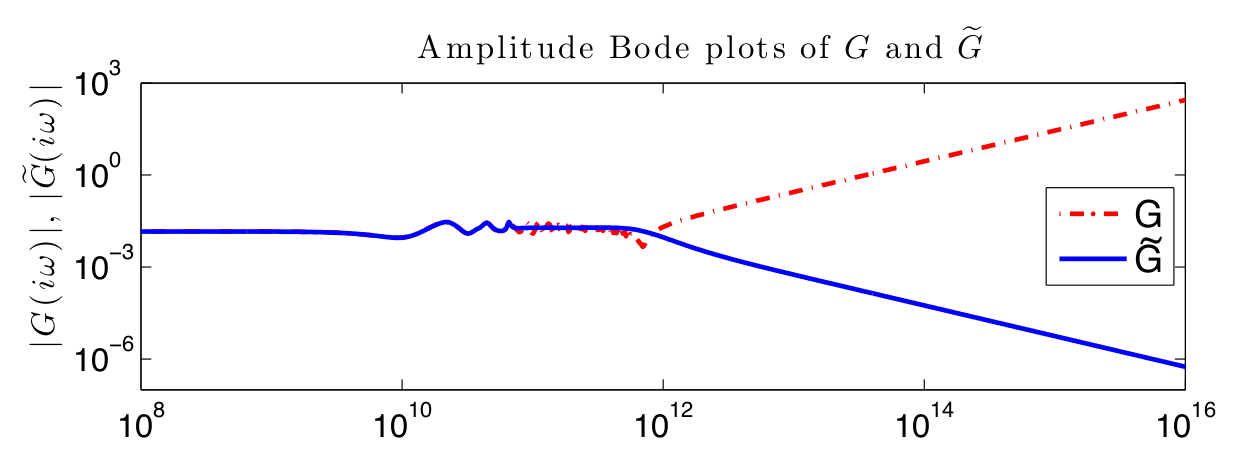
\includegraphics[width=\textwidth]{GugSW-properimproper}

	The general problem is:
	\begin{itemize}
		\item the transfer function can have an improper part (frequency domain)
		\item the system differentiates the input (time domain)
	\end{itemize}

	The general approach is:
	\begin{enumerate}
		\item Project the DAE onto the part that is an ODE, i.e. a standard state space system
		\item Keep the remainder, i.e. the algebraic or improper part, as it is 
	\end{enumerate}
	This means: \emph{no model reduction on the algebraic part!}

\subsection{Balanced Truncation for Navier-Stokes Systems}
  We consider linearized Navier-Stokes equations:
	\begin{align*}
		M \dot v(t) &=  A_1v(t) + J^T p(t) + B_1 u(t), \\
		Jv(t) &= 0, \\
		y(t) &= C_1v(t).
	\end{align*}

\begin{itemize}
	\item $v(t) \in \Rn$: one system's state (velocity)
	\item $p(t) \in \Rp$: another system's state (pressure)
	\item $u(t) \in \Rm$: the input or control
	\item $y(t) \in \Rq$: the output or measurements
	\item $M \in \Rnn$ is the mass matrix (symmetric positive definite)
	\item $A_1 \in \Rnn$: the system matrix
	\item $J \in \Rpn$ is another system matrix (full rank)
	\item $B_1 \in \Rnm$: an input matrix
	\item $B_2 \in \Rpm$: another input matrix
	\item $C_1 \in \Rqn$: an output matrix
	\item $C_2 \in \mathbb R^{q\times p} $: another output matrix
\end{itemize}

Note that this is an \eabcsys~with
\begin{equation*}
	E:= \begin{bmatrix} M & 0 \\ 0 & 0 \end{bmatrix}, \quad
	A:= \begin{bmatrix} A_1 & -J \\ J^T & 0 \end{bmatrix}, \quad
	B:= \begin{bmatrix} B_1 \\ B_2\end{bmatrix}, \quad \text{and}\quad
	C:= \begin{bmatrix} C_1 & C_2 \end{bmatrix}.
\end{equation*}

Simplifying properties and assumptions:
\begin{itemize}
	\item linearity -- the Navier-Stokes equations are nonlinear
	\item stability -- this is only true for slowly moving flows
	\item ``$B_2=0$'' and ``$C_2=0$'': the improper part is zero
\end{itemize}

\subsection{Decoupling Differential and Algebraic Parts}
Consider the projector
\begin{equation*}
	P := I - M^{-1}J^\trp(JM^{-1}J^\trp)^{-1}J
\end{equation*}
and see that with $v=Pv + (I-P)v=:v_d + v_a$ the system writes as
	\begin{align*}
		M \dot v_d(t) &=  P^\trp A_1v_d (t) + P^\trp A_1v_a(t)+  P^\trp B_1 u(t), \\
		v_a(t) &= -M^{-1}J^\trp(JM^{-1}J^\trp)^{-1}JB_2u(t), \\
		p(t) &= -(JM^{-1}J^\trp)^{-1}\bigl[ JM^{-1}[A(v_a(t)+v_d(t))+B_1u(t)]-B_2\dot u(t)\bigr], \\
		y(t) &= C_1v_d(t)+C_1v_a(t) + C_2p(t),
	\end{align*}
which, since $v_a$ and $p$ depend linearly on $v_d$, $u$, and $\dot u$ is an $\eabcdsys$ system with
\begin{align*}
	E &:= M, \\
	A &:= P^\trp A, \\
	B &:= P^\trp [B_1 - AM^{-1}J^\trp(JM^{-1}J^\trp)^{-1}JB_2], \\
	C &:= C_1 - C_2(JM^{-1}J^\trp)^{-1}JM^{-1}A, \\
	D &:= D_1 + D_2,
\end{align*}
with
\begin{align*}
	D_1&:=-C_1M^{-1}J^\trp(JM^{-1}J^\trp)^{-1}JB_2 + C_2(JM^{-1}J^\trp)^{-1}\bigl[ JM^{-1}AM^{-1}J^\trp(JM^{-1}J^\trp)^{-1}JB_1 \\
	D_2&:=-C_2(JM^{-1}J^\trp)^{-1}B_2\frac{\inva{}}{\inva t}.
\end{align*}
Note that 
\begin{itemize}
	\item The transfer function is given as $G=C(sE-A)^{-1}B+D_1+sD_2$
	\item if $B_2$ or $C_2$ is zero, then $D_2$ is zero,
		\begin{itemize}
			\item no $\dot u$ in the output
			\item no obviously improper part $sD_2$ in $G$
		\end{itemize}
	\item if $B_2$ is zero, then $D_1$, $D_2=0$
		\begin{itemize}
			\item we obtain a standard \eabcsys~system
			\item no improper parts in $G$
		\end{itemize}
\end{itemize}

We assume that $B_2$ and $C_2$ are zero. Then we have a standard \eabcsys, with
\begin{align*}
	E &:= M, \\
	A &:= P^\trp A, \\
	B &:= P^\trp B_1, \\
	C &:= C_1 .
\end{align*}
If we want to apply Balanced Truncation, we need to cope with the following difficulties:
\begin{itemize}
	\item The system is not minimal
		\begin{itemize}
			\item[$\to$] this is automatically \emph{fixed} by BT, if we can find the right solutions of the nonregular Lyapunov equations like 
				\begin{equation*}
					MXP^TA + APXM + P^\trp B B^\trp P = 0.
				\end{equation*}
		\end{itemize}
	\item The system is not stable
		\begin{itemize}
			\item[$\to$] Combine BT with \emph{LQG}-stabilization \cite{morBenH15}
		\end{itemize}
	\item Explicit computation of projectors is not possible for large scale systems
		\begin{itemize}
			\item[$\to$] use algorithms that do not need $P$ explicitly \cite{morHeiSS08, morBenH15, morGugSW13}
		\end{itemize}
\end{itemize}
Add slides
\begin{enumerate}
	\item setup cylinderwake
	\item Bode plot for various $\kappa$
	\item results
\end{enumerate}

